\documentclass[conference]{IEEEtran}
\usepackage{amsmath,amssymb,amsfonts}
\usepackage{graphicx}
\usepackage{booktabs}
\usepackage{cite}
\usepackage{url}
\usepackage{textcomp}
\usepackage{xcolor}
\usepackage[section]{placeins}

\graphicspath{{figures/}{../figures/}{./}}

\begin{document}

\title{Detectability Margins for Meter-Aware Charge-Injection Monitoring in Residential Energy Storage Agents}

\author{\IEEEauthorblockN{Magne Dina Neves}
\IEEEauthorblockA{Faculty of Science and Technology\\
University of Macau\\
Macao SAR, China\\
Email: (add institutional email before submission)}
}

\maketitle

\begin{abstract}
Residential battery agents report state of charge (SoC) and power to an energy storage management system (ESMS) and accept remote charge commands. An attacker who forges both reports consistently can defeat any residual that depends only on those fields. An independent household net meter restores observability of unauthorized charge injection, but that recovery is not automatic: it depends on meter noise, load-estimate error, and whether the load estimate itself is compromised. This paper treats the problem as a detectability and design study rather than a new detector. On a Python cyber-physical testbed we use held-out calibration (seeds 42--51) and held-out evaluation (seeds 52--71), report 14-day benign alarms-per-day, compare S2 threshold / EWMA / CUSUM at matched false-alarm operating points, sweep minimum detectable injection power (MDIP) down to $0.05\,\mathrm{kW}$ across meter and load-estimate noise classes, and quantify collapse under partial load-estimate spoofing (A6). Across the tested noise grid, MDIP at detection rate $\ge 0.9$ is at most $0.1\,\mathrm{kW}$; at nominal noise a $0.05\,\mathrm{kW}$ trickle is still detected but with multi-hour delay (about $0.1\,\mathrm{kWh}$ of undetected energy transfer before alarm). S2 detection collapses only when the load estimate is fully steered to hide injection ($\alpha=1$), which requires read-only access to the meter stream but not the ability to forge it.
\end{abstract}

\begin{IEEEkeywords}
Battery energy storage, cyber-physical security, Energy Internet of Things, false data injection, detectability, net metering, CUSUM.
\end{IEEEkeywords}

\section{Introduction}
Cloud-managed residential batteries expose an Energy IoT path: an agent reports SoC and power and receives charge or discharge setpoints. Compromising that path enables integrity attacks without BMS cell-sensor access. Prior work has studied BMS voltage/current FDIAs~\cite{trevizan2022,zhuang2021,obrien2023,obrien2024}, device-side setpoint inspection~\cite{hossen2022}, and false SoC reports for charging priority~\cite{elshazly2024}. Less attention is paid to a design question for ESMS operators: how small an injection remains detectable once a meter channel is added, and how far a soft load estimate can be corrupted before that channel fails.

If a detector uses only reported SoC and reported battery power, an attacker who sets both fields can keep them Coulomb-consistent and drive the residual to noise. Pairing that limit with an independent meter is useful only if the resulting detectability margins are quantified. This paper therefore emphasizes MDIP, long-horizon false alarms, classical baselines, and a load-estimate adversary, not a named algorithm.

Contributions:
\begin{enumerate}
\item Held-out calibration with explicit coefficients and 14-day benign alarms-per-day on held-out seeds.
\item S2 baseline comparison (raw threshold, EWMA, CUSUM) at matched false-alarm operating points, including gradual injection.
\item MDIP curves under meter-noise and load-estimate-noise classes for a stealth consistent injector (A5).
\item Partial load-estimate compromise sweep (A6) showing when S2 collapses.
\end{enumerate}

\section{Related Work}
Trevizan \textit{et al.} survey BESS cyber-physical security and highlight ESMS as an outward-facing subsystem~\cite{trevizan2022}. BMS-layer FDIA detection with Kalman residuals and CUSUM is mature~\cite{obrien2023,obrien2024}. Zhuang and Liang study SoC FDIAs in distribution networks~\cite{zhuang2021}. Self-protective inverters inspect malicious setpoints at the device~\cite{hossen2022}. Lying-SoC charging work focuses on unfair priority with learning detectors~\cite{elshazly2024}. Fan \textit{et al.} address resilient ESS secondary control under FDI~\cite{fan2024}. We study residential ESMS monitoring margins with and without an independent meter channel.

\section{System and Threat Model}
\subsection{Physical and Cyber Paths}
The plant is a 10\,kWh battery with Coulomb counting ($\eta_c=\eta_d=0.95$, $\Delta t=60\,\mathrm{s}$). House load $P_L>0$ consumes AC power. Battery power $P_B$ is positive when discharging. Grid import satisfies
\begin{equation}
P_G = P_L - P_B.
\end{equation}
The agent reports $(s^{\mathrm{rep}}, P_B^{\mathrm{rep}})$ to the ESMS. An independent meter reports noisy $P_G^{\mathrm{meas}}$. The ESMS also holds a load estimate $P_L^{\mathrm{est}}$ (for example from a home energy monitor).

\subsection{Trust Assumptions (deployment)}
We separate integrity from confidentiality on the meter path:
\begin{itemize}
\item \textbf{Meter integrity.} The ESMS trusts $P_G^{\mathrm{meas}}$ as authenticated (utility/AMI path or sealed meter). The attacker cannot forge or replace the meter sample used by the detector.
\item \textbf{Meter confidentiality (optional for A6).} A home-network compromise may grant \emph{read-only} access to the local meter data stream (e.g., Modbus/Zigbee/LAN tap). Reading $P_G^{\mathrm{meas}}$ does not imply write access to the ESMS meter input.
\item \textbf{Load estimate is soft.} $P_L^{\mathrm{est}}$ is untrusted unless independently attested. Soft monitors and cloud load models are assumed forgeable once the gateway is owned.
\end{itemize}
Forging the meter reading itself (integrity break) is out of scope. With read-only meter access, A6 can null $r^{(2)}$ by poisoning $P_L^{\mathrm{est}}$ alone; without that read, the attacker cannot target $P_G^{\mathrm{meas}}+P_B^{\mathrm{rep}}$ exactly and A6 overstates capability.

\subsection{Compromise Scenario}
\textbf{Baseline (A1--A5):} compromised agent credential or home gateway; rewrite agent telemetry; inject charge commands; no meter forge; no assumption of meter read.
\textbf{Extended (A6):} baseline capabilities plus read-only meter stream access and write access to $P_L^{\mathrm{est}}$.

\subsection{Attacks}
\begin{itemize}
\item A1: constant SoC bias.
\item A2: slow SoC ramp.
\item A3: charge injection with under-reported power.
\item A4: coordinated ramp plus injection with stronger power hiding.
\item A5: stealth consistent dual spoof (inject while reporting idle power and a SoC trajectory integrated from that forged power).
\item A6: A5-style dual spoof plus partial load-estimate compromise using the read meter sample:
$P_L^{\mathrm{est}}\leftarrow(1-\alpha)P_L^{\mathrm{est}}+\alpha(P_G^{\mathrm{meas}}+P_B^{\mathrm{rep}})$, $\alpha\in[0,1]$.
\end{itemize}

\section{Detection Method}
\subsection{S1: ESMS-only energy balance}
\begin{equation}
r^{(1)}_k = \Delta s^{\mathrm{rep}}_k - f(P_B^{\mathrm{rep}}; E_{\mathrm{nom}},\eta),
\end{equation}
where $f$ is the Coulomb-counting map.

\subsection{S2: meter cross-check}
\begin{equation}
\hat{P}_B = P_L^{\mathrm{est}} - P_G^{\mathrm{meas}}, \qquad
r^{(2)}_k = \hat{P}_B - P_B^{\mathrm{rep}}.
\end{equation}
Under A6, the honest residual is scaled by $(1-\alpha)$ in the noise-free model, so detectability shrinks as $\alpha\to 1$.

\subsection{Baselines and fuse}
On each residual we evaluate raw absolute threshold, EWMA ($\alpha_{\mathrm{ew}}=0.2$), and two-sided CUSUM. The OR fuse alarms if S1-CUSUM or S2-CUSUM fires.

\subsection{Observation (ESMS-only stealth boundary)}
In the noise-free model, if an alarm depends only on $r_k=\Delta s^{\mathrm{rep}}_k-f(P_B^{\mathrm{rep}}_k)$ and the attacker chooses both reports, setting $\Delta s^{\mathrm{rep}}_k=f(P_B^{\mathrm{rep}}_k)$ yields $r_k=0$. This is an observability remark, not a formal lemma. Meter-inferred $\hat{P}_B$ can still expose injection through $r^{(2)}$ when $P_L^{\mathrm{est}}$ is not fully compromised.

\subsection{Held-out calibration (self-contained)}
Calibration uses benign windows on seeds $\{42,\ldots,51\}$ only. Let $\sigma_1=\mathrm{std}(r^{(1)})$ and $\sigma_2=\mathrm{std}(r^{(2)})$. Parameters are
\begin{align}
\tau_1 &= \max(0.004,\,5\sigma_1),\quad
\nu_1 = \max(10^{-4},\,0.5\sigma_1),\quad
H_1 = \max(0.006,\,4\sigma_1),\\
\tau_2 &= \max(0.25,\,4\sigma_2),\quad
\nu_2 = \max(0.03,\,0.5\sigma_2),\quad
H_2 = \max(1.0,\,8\sigma_2),
\end{align}
with EWMA thresholds $3\sigma_1$ and $3\sigma_2$ (floored at $0.002$ and $0.15$). If needed, $H_2$ is raised on calibration seeds until mean S2-CUSUM alarms/day $\le 0.1$. Evaluation seeds $\{52,\ldots,71\}$ are never used for threshold selection. Empirically, $\sigma_1\approx 1.41\times 10^{-3}$, $\sigma_2\approx 0.0988$, and $H_2=1.0$ already met the calibration APD target.

\section{Experimental Setup}
Python 3.12 testbed on a personal computer. Agent/meter noise, meter dropouts, and load-estimate noise are enabled. Scenario runs: 720 steps (12\,h), attack start at step 180, 20 held-out eval seeds. Seeds control the random draws for meter noise, load-estimate noise, and meter dropout events; the underlying load and battery schedules are identical across seeds. Long false-alarm study: 14 days $\times$ 10 held-out seeds at 1-min steps. MDIP sweep: sustained $|P_{\mathrm{inj}}|\in\{0.05,0.1,0.15,0.2,0.5,1,2,3\}\,\mathrm{kW}$ under meter noise $\{0.02,0.05,0.15\}\,\mathrm{kW}$ and load-estimate noise $\{0.05,0.08,0.20\}\,\mathrm{kW}$. A6 sweeps $\alpha\in\{0,0.25,0.5,0.75,0.9,1\}$ under the read-only meter assumption above.

\section{Results}
\subsection{Held-out detection rates}
Table~\ref{tab:mc} summarizes detection on eval seeds. S1 catches inconsistent spoofs. A5 largely defeats S1 (rate $0.15$) but not S2 (rate $1.0$, mean delay $0$). After tightening, S2 does not raise non-injection alerts on A1/A2 (rate $0$). Fig.~\ref{fig:a5} shows representative time traces for A5: the S1 residual stays near noise while the S2 residual responds when the meter implies unauthorized charging.

\begin{figure}[t]
\centering
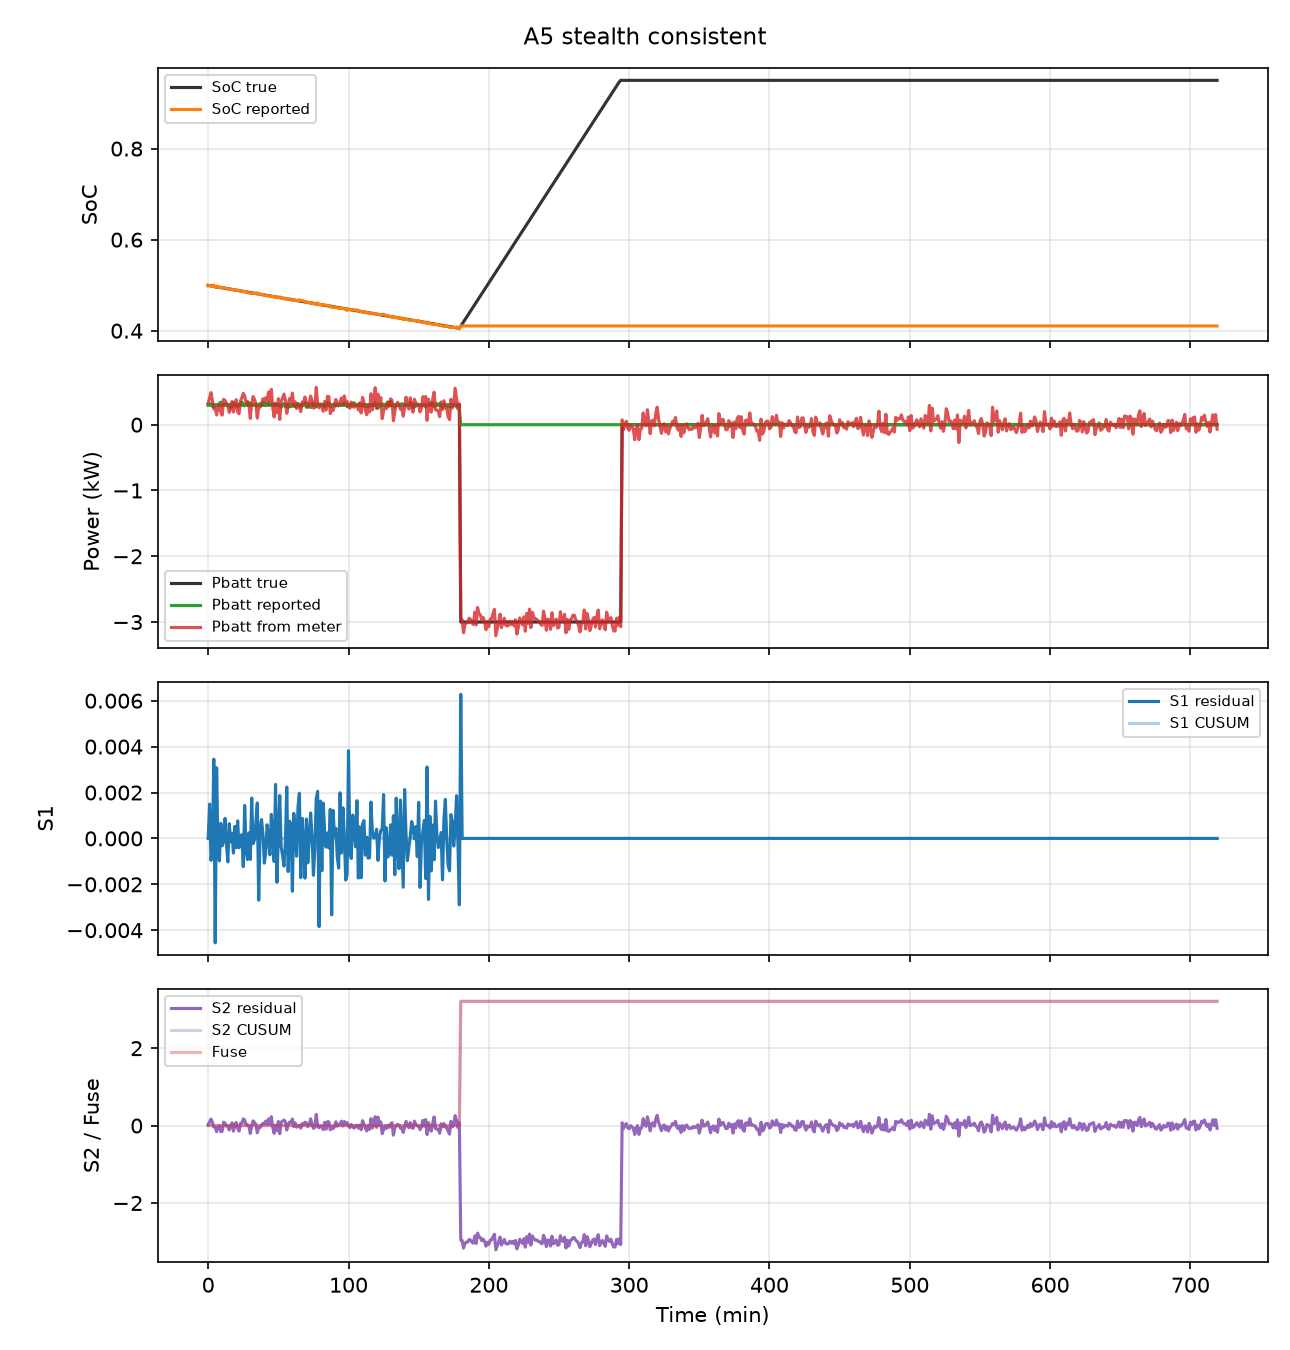
\includegraphics[width=\columnwidth]{A5_stealth_consistent.png}
\caption{Time traces for the A5 stealth consistent dual spoof: the S1 energy-balance residual remains quiet while the S2 meter residual responds to unauthorized charging.}
\label{fig:a5}
\end{figure}

\begin{table}[t]
\centering
\caption{Held-out detection (20 seeds, 12\,h). Rate / mean delay (min). Fuse = S1 OR S2 CUSUM.}
\label{tab:mc}
\setlength{\tabcolsep}{2.5pt}
\resizebox{\columnwidth}{!}{%
\begin{tabular}{@{}lccc@{}}
\toprule
Scenario & S1 CUSUM & S2 CUSUM & Fuse \\
\midrule
A1 SoC bias & 1.00 / 0.0 & 0.00 / -- & 1.00 / 0.0 \\
A2 SoC ramp & 1.00 / 39.1 & 0.00 / -- & 1.00 / 39.1 \\
A3 cmd inject & 1.00 / 1.3 & 1.00 / 0.0 & 1.00 / 0.0 \\
A4 coordinated & 1.00 / 1.4 & 1.00 / 0.0 & 1.00 / 0.0 \\
A5 stealth consist. & 0.15 / -- & 1.00 / 0.0 & 1.00 / 0.0 \\
A6 ($\alpha=0.5$) & 0.15 / -- & 1.00 / 0.0 & 1.00 / 0.0 \\
\bottomrule
\end{tabular}%
}
\end{table}

\subsection{Long-horizon false alarms}
Table~\ref{tab:fpr} reports mean alarms per day over 14-day benign runs on held-out seeds. All channels stay near or below the $0.1$/day design target; the fuse averages $0.086$/day.

\begin{table}[t]
\centering
\caption{Mean alarms per day on 14-day benign held-out runs (10 seeds).}
\label{tab:fpr}
\setlength{\tabcolsep}{3pt}
\begin{tabular}{@{}lcccc@{}}
\toprule
 & S1 th & S1 CU & S2 th & S2 CU & Fuse \\
\midrule
Alarms/day & 0.007 & 0.043 & 0.071 & 0.043 & 0.086 \\
\bottomrule
\end{tabular}
\end{table}

\subsection{S2 baselines at matched FPR}
At the calibrated operating point, threshold, EWMA, and CUSUM all achieve A5 detection rate $1.0$ with near-zero 12\,h benign FPR (Fig.~\ref{fig:base}). For gradual $0.5\,\mathrm{kW}$ injection, mean delays are $0.4$\,min (threshold), $1.9$\,min (CUSUM), and $3.8$\,min (EWMA). Thus CUSUM is not claimed as faster here; it is retained as a classical cumulative monitor alongside the raw mismatch threshold.

\begin{figure}[t]
\centering
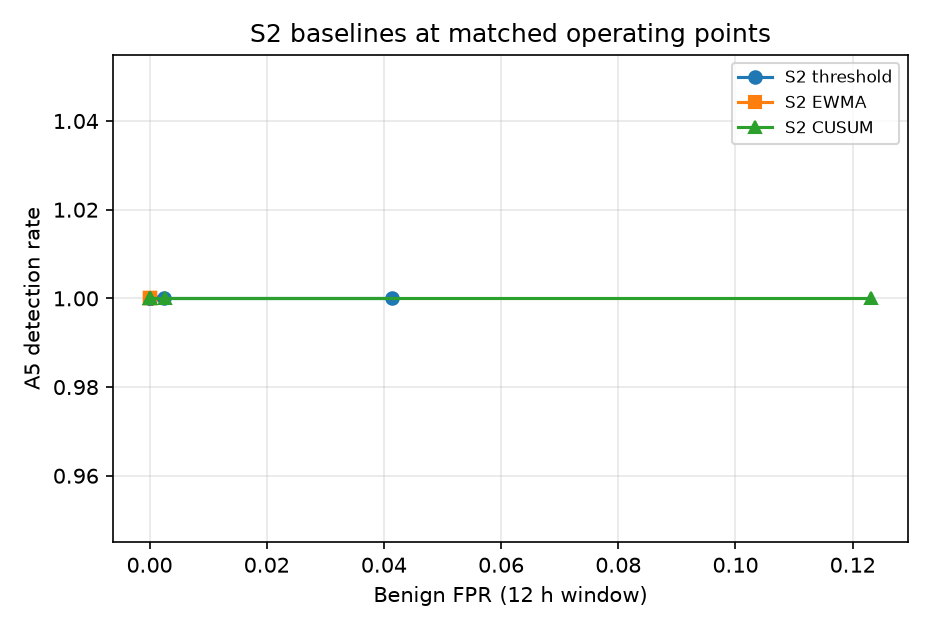
\includegraphics[width=\columnwidth]{baseline_roc.png}
\caption{Operating curves for three S2 residual processors (absolute threshold, EWMA, CUSUM): A5 detection rate versus benign false-positive rate under a common threshold-scale sweep.}
\label{fig:base}
\end{figure}

\subsection{Minimum detectable injection power}
Fig.~\ref{fig:mdip} shows detection rate versus sustained $|P_{\mathrm{inj}}|$ for three meter-noise levels at load-estimate noise $0.08\,\mathrm{kW}$. With the finer grid, MDIP at detection rate $\ge 0.9$ is $0.05\,\mathrm{kW}$ for eight of nine noise pairs and $0.1\,\mathrm{kW}$ for the remaining pair (meter $\sigma=0.02$, load-est.\ $\sigma=0.05$), where $0.05\,\mathrm{kW}$ yields rate $0.88$. At nominal noise ($0.05$/$0.08\,\mathrm{kW}$), mean S2-CUSUM delay grows sharply as injection shrinks: $127$\,min at $0.05\,\mathrm{kW}$, $24$\,min at $0.1\,\mathrm{kW}$, $6.6$\,min at $0.2\,\mathrm{kW}$, and $1.9$\,min at $0.5\,\mathrm{kW}$. Thus a $50\,\mathrm{W}$ trickle remains detectable in this model, but not promptly.

\begin{figure}[t]
\centering
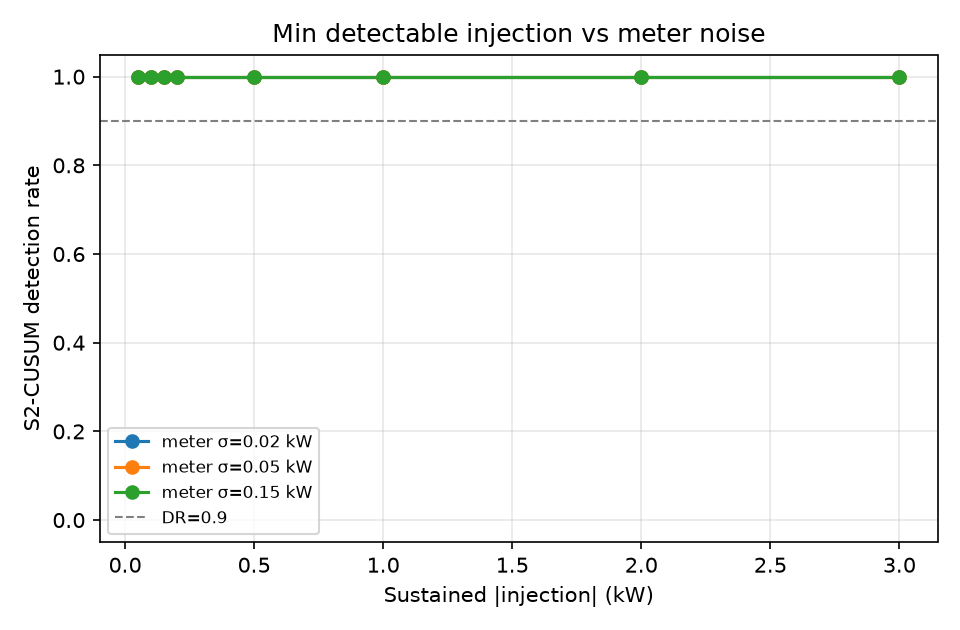
\includegraphics[width=\columnwidth]{mdip_curves.png}
\caption{Detection rate of the S2 CUSUM versus sustained charge-injection magnitude for three meter-noise standard deviations (load-estimate noise fixed at $0.08\,\mathrm{kW}$).}
\label{fig:mdip}
\end{figure}

\subsection{Load-estimate adversary (A6)}
\begin{figure}[!t]
\centering
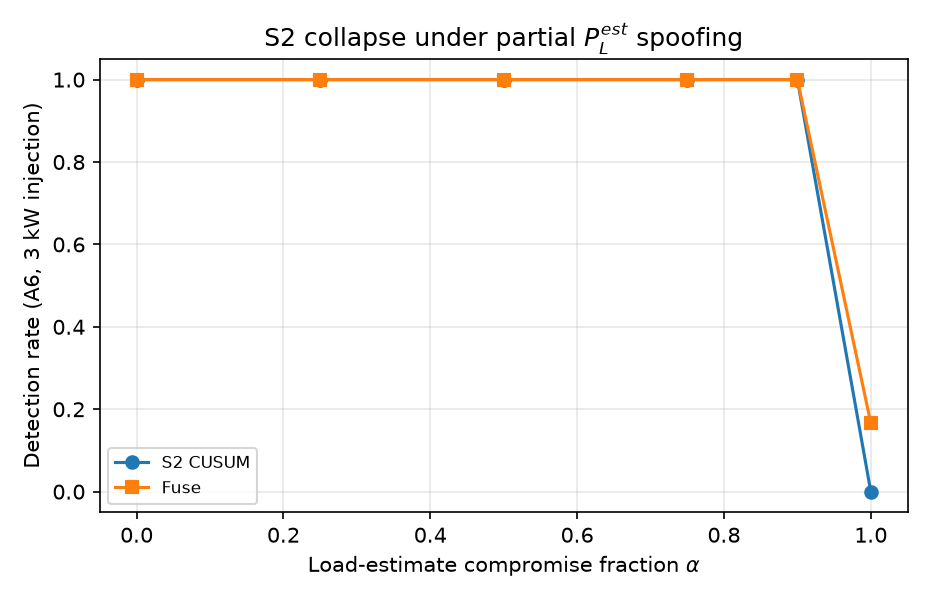
\includegraphics[width=0.92\columnwidth]{a6_alpha_sweep.png}
\caption{Detection rate of S2 CUSUM and the S1/S2 fuse versus load-estimate compromise fraction $\alpha$ under attack A6 ($3\,\mathrm{kW}$ sustained injection, read-only meter access).}
\label{fig:a6}
\end{figure}
Fig.~\ref{fig:a6} shows S2 detection versus $\alpha$ for a $3\,\mathrm{kW}$ consistent injector under read-only meter access. Detection remains $1.0$ through $\alpha=0.9$ (delay rises to $3.3$\,min) and collapses at $\alpha=1.0$ (S2 rate $0$; fuse rate $0.17$ from residual S1 hits). This matches the $(1-\alpha)$ residual scaling: full compromise of $P_L^{\mathrm{est}}$ closes the meter cross-check without forging $P_G^{\mathrm{meas}}$.

\FloatBarrier
\section{Discussion and Limitations}
The study quantifies when a meter channel helps and when it fails. Useful margins in this testbed: MDIP $\le 0.1\,\mathrm{kW}$ under the tested noise grid, with a clear delay penalty for trickle injection, and S2 survival until near-complete load-estimate spoofing given meter read access. Raw threshold can outperform CUSUM on delay for strong sustained bias; the contribution is not ``CUSUM wins.'' A6 should be read as a home-LAN confidentiality break plus soft load-estimate write, not as a meter integrity break.

Detectability at $0.05\,\mathrm{kW}$ does not imply timely containment. At nominal noise the mean S2-CUSUM delay is about $127$\,min, so before an alarm an adversary can move on the order of $0.05\,\mathrm{kW}\times 2\,\mathrm{h}\approx 0.1\,\mathrm{kWh}$ of unauthorized energy (energy theft or billing mismatch on a $10\,\mathrm{kWh}$ pack) and impose extra cycling that contributes to wear. Operators who find that delay window unacceptable may need tighter residual processors, a secondary energy-accumulation monitor, or a shorter sample interval. The immediate next step is to replay the same held-out calibration and evaluation protocol on public residential load traces (e.g., Pecan Street) or a hardware testbed, to test whether MDIP and alarms/day transfer beyond Gaussian synthetic loads.

Limitations: synthetic schedules, Coulomb-counting plant, Gaussian noise, no field packet capture, and no HIL in the present study. Adaptive load estimators (Kalman / GLRT) may lower residual variance and MDIP further; they are left for Phase~2. Meter-forging adversaries remain out of scope.

\section{Conclusion}
For a stealth consistent charge-injection adversary on the agent path, we characterized detectability of a meter-aware residual under meter noise and load-estimate error, compared classical S2 baselines at matched false-alarm points, and showed S2 collapse under full load-estimate compromise when the attacker can read but not forge the meter. Claims match the held-out numbers above; the methods are classical, and the contribution is the margin analysis.

\begin{thebibliography}{00}
\bibitem{trevizan2022}
R.~D. Trevizan, J.~Obert, V.~De~Angelis, T.~A. Nguyen, V.~S. Rao, and B.~R. Chalamala, ``Cyberphysical Security of Grid Battery Energy Storage Systems,'' \textit{IEEE Access}, vol.~10, pp.~59675--59721, 2022, doi: 10.1109/ACCESS.2022.3178987.

\bibitem{zhuang2021}
P.~Zhuang and H.~Liang, ``False Data Injection Attacks Against State-of-Charge Estimation of Battery Energy Storage Systems in Smart Distribution Networks,'' \textit{IEEE Trans. Smart Grid}, vol.~12, no.~3, pp.~2566--2577, May 2021, doi: 10.1109/TSG.2020.3042926.

\bibitem{obrien2023}
V.~O'Brien, V.~S. Rao, and R.~D. Trevizan, ``Detection of False Data Injection Attacks in Battery Stacks Using Input Noise-Aware Nonlinear State Estimation and Cumulative Sum Algorithms,'' \textit{IEEE Trans. Ind. Appl.}, vol.~59, no.~6, Nov./Dec. 2023, doi: 10.1109/TIA.2023.3308548.

\bibitem{obrien2024}
V.~A. O'Brien, V.~S. Rao, and R.~D. Trevizan, ``Online and Offline Identification of False Data Injection Attacks in Battery Sensors Using a Single Particle Model,'' \textit{IEEE Open Access J. Power Energy}, 2024, doi: 10.1109/OAJPE.2024.3493757.

\bibitem{hossen2022}
T.~Hossen, M.~Gursoy, and B.~Mirafzal, ``Self-Protective Inverters Against Malicious Setpoints Using Analytical Reference Models,'' \textit{IEEE J. Emerg. Sel. Topics Ind. Electron.}, vol.~3, no.~4, pp.~871--877, Oct. 2022, doi: 10.1109/JESTIE.2022.3199672.

\bibitem{elshazly2024}
A.~A. El-Shazly \textit{et al.}, ``False Data Injection Attacks on Reinforcement Learning-Based Charging Coordination in Smart Grids and a Countermeasure,'' \textit{Appl. Sci.}, vol.~14, no.~23, Art.~no.~10874, 2024, doi: 10.3390/app142310874.

\bibitem{fan2024}
S.~Fan, D.~Yue, H.~Yan, and C.~Deng, ``Distributed Round-Robin Protocol-Based Secondary Control for ESSs Under FDI Attacks,'' \textit{IEEE Trans. Ind. Electron.}, vol.~71, no.~12, pp.~16493--16502, Dec. 2024, doi: 10.1109/TIE.2024.3390733.
\end{thebibliography}

\end{document}
